% fig_arch_v7 (column width): the detector as a network diagram. Redrawn from fig_arch.tex with the explanatory sentences moved
% to the caption (fig_arch_v7_caption.txt). Source of every detail: results/research/retouch_unified_20260929/train_ru5.py
% (CLIP ViT-L/14 frozen; LoRA r=16 on q/k/v/out projections of all 24 blocks; heads on the pooled feature: z_f, z_b, 4 presence,
% 4 quantity; evidence = linear 1024->1 on the 256 patch tokens -> 16x16 map, trained against the exact footprint M;
% consistency term L_cons on the paired smoothed view x_s). Thumbnails: img/x.png, img/xs.png, img/ev_grid.png, img/footprint16.png.
\documentclass[tikz,border=1.5pt]{standalone}
% Shared visual language of the TikZ figures (fig_arch, fig_system, fig_protocol, fig_exposure, fig_explain_layers).
% Colours are the palette of docs/paper_v2/figstyle.py: house blue for our model, Okabe-Ito green / vermillion for correct /
% error, light fills by stage type (network, code, language model, check, fallback, input/output), thin dark arrows.
% Text: TeX Gyre Heros (Helvetica metrics), 7 pt body; tensor shapes in DejaVu Sans Mono 5.5 pt.
\usepackage{fontspec}
\setsansfont{texgyreheros}[Extension=.otf,UprightFont=*-regular,BoldFont=*-bold,ItalicFont=*-italic,BoldItalicFont=*-bolditalic]
\setmonofont{DejaVuSansMono}[Path=/usr/share/fonts/truetype/dejavu/,Extension=.ttf,BoldFont=*-Bold,Scale=0.92]
\renewcommand{\familydefault}{\sfdefault}
\usepackage{amsmath}
\usepackage[italic]{mathastext}
\usetikzlibrary{positioning,arrows.meta,fit,backgrounds,calc,shapes.misc,decorations.pathreplacing}

% ---- palette (figstyle.py) -----------------------------------------------------------------------------------------
\definecolor{ink}{HTML}{222222}
\definecolor{muted}{HTML}{6B6B6B}
\definecolor{gridc}{HTML}{E5E5E5}
\definecolor{ours}{HTML}{0F4D92}     % house blue: our model, trainable parts
\definecolor{oursarm}{HTML}{5B9BD5}
\definecolor{okc}{HTML}{009E73}      % genuine / correct
\definecolor{errc}{HTML}{D55E00}     % forged / error
\definecolor{amber}{HTML}{C98A00}    % language model (deck palette)
\definecolor{plum}{HTML}{A8538A}     % checks
\definecolor{truth}{HTML}{56B4E9}    % ground-truth footprint
\definecolor{hilite}{HTML}{FFD700}
% light fills by stage type
\definecolor{fNet}{HTML}{E2EBF6}
\definecolor{fCode}{HTML}{DFF2EA}
\definecolor{fLLM}{HTML}{FCEFD6}
\definecolor{fChk}{HTML}{F6E6F0}
\definecolor{fFall}{HTML}{FBE4D8}
\definecolor{fIO}{HTML}{F4F4F4}

\newcommand{\bodyfont}{\fontsize{7}{8.2}\selectfont}
\newcommand{\smallfont}{\fontsize{6.2}{7.2}\selectfont}
\newcommand{\shp}[1]{{\fontsize{5.6}{6.4}\selectfont\ttfamily\color{muted}#1}}   % tensor-shape annotation
\newcommand{\hd}[1]{{\bfseries #1}}

\tikzset{
  every picture/.style={line width=0.5pt, font=\bodyfont, >={Stealth[length=3.4pt,width=2.8pt]}},
  stage/.style={rounded corners=2.2pt, draw=#1!75!black, line width=0.5pt, align=center, inner sep=2.6pt},
  net/.style={stage=ours, fill=fNet},
  code/.style={stage=okc, fill=fCode},
  llm/.style={stage=amber, fill=fLLM},
  chk/.style={stage=plum, fill=fChk},
  fall/.style={stage=errc, fill=fFall},
  io/.style={stage=muted, fill=fIO},
  plain/.style={rounded corners=2.2pt, draw=ink!55, fill=white, align=center, inner sep=2.6pt},
  flow/.style={->, draw=ink, line width=0.55pt},
  tflow/.style={->, draw=ink, line width=0.55pt, dash pattern=on 2.2pt off 1.4pt},   % training-time only
  errflow/.style={->, draw=errc, line width=0.6pt},
  okflow/.style={->, draw=okc, line width=0.6pt},
  thumb/.style={inner sep=0pt, draw=muted, line width=0.35pt},
  lbl/.style={font=\smallfont, text=ink, align=center, inner sep=1pt},
  note/.style={font=\smallfont, text=muted, align=center, inner sep=1pt},
  badge/.style={rounded corners=5pt, draw=#1, fill=white, line width=0.5pt, font=\smallfont\bfseries, text=#1, inner xsep=3pt, inner ysep=1.6pt},
}

\newcommand{\tinyf}{\fontsize{5.2}{6}\selectfont}
\newcommand{\vdotsdraw}[1]{\foreach \d in {-0.08,0,0.08}{\fill[muted] ($(#1)+(0,\d)$) circle (0.5pt);}}
% a transformer block: q k v o squares, each with a LoRA chip, then the frozen MLP slot
\newcommand{\block}[2]{% y, number
  \node[draw=ink!40, fill=white, rounded corners=1.2pt, minimum width=2.1cm, minimum height=0.4cm] at (2.5,#1) {};
  \node[font=\tinyf, text=muted, inner sep=0pt] at (1.6,#1) {#2};
  \foreach \k/\n in {0/q,1/k,2/v,3/o}{
    \node[draw=ink!45, fill=fIO, line width=0.4pt, minimum size=0.25cm, inner sep=0pt, font=\tinyf\ttfamily, text=ink] (sq) at (1.9+\k*0.3,#1) {\n};
    \fill[ours] ($(sq.north east)+(-0.02,-0.0)$) rectangle ++(-0.12,0.07);}
  \node[draw=ink!30, fill=fIO, rounded corners=0.8pt, minimum width=0.42cm, minimum height=0.25cm, inner sep=0pt, font=\tinyf, text=muted] at (3.22,#1) {MLP};}
% sparkle badge (same glyph as fig_exposure_v7)
\newcommand{\sparkle}[3]{% x y r
  \fill[oursarm] (#1,#2) circle (#3);
  \fill[white] ($(#1,#2)+(0,0.68*#3)$) -- ($(#1,#2)+(0.22*#3,0.22*#3)$) -- ($(#1,#2)+(0.68*#3,0)$) -- ($(#1,#2)+(0.22*#3,-0.22*#3)$)
     -- ($(#1,#2)+(0,-0.68*#3)$) -- ($(#1,#2)+(-0.22*#3,-0.22*#3)$) -- ($(#1,#2)+(-0.68*#3,0)$) -- ($(#1,#2)+(-0.22*#3,0.22*#3)$) -- cycle;}
\begin{document}
\begin{tikzpicture}[x=1cm,y=1cm]
% ---------------------------------------------------------------- inputs
\node[thumb] (x) at (0.55,2.45) {
\includegraphics[width=0.9cm]{img/x.png}};
\node[lbl, anchor=north, inner sep=1.5pt] at (x.south) {face crop $x$};
\node[thumb, draw=ours, dash pattern=on 1.6pt off 1pt, line width=0.5pt] (xs) at (0.55,0.75) {
\includegraphics[width=0.9cm]{img/xs.png}};
\sparkle{0.88}{1.08}{0.1}
\node[lbl, anchor=north, inner sep=1.5pt] at (xs.south) {$x_s$: smoothed};
\node[note, anchor=south, inner sep=1pt, font=\tinyf] at ([yshift=0.5pt]xs.north) {training only};

% ---------------------------------------------------------------- shared backbone
\node[net, minimum width=2.5cm, minimum height=3.35cm] (vit) at (2.5,1.5) {};
\node[anchor=north, font=\smallfont\bfseries, text=ours, inner sep=0pt] at ([yshift=-2.5pt]vit.north) {CLIP ViT-L/14};
\node[anchor=north, note, font=\tinyf, inner sep=0pt] at ([yshift=-10pt]vit.north) {shared by $x$ and $x_s$};
\block{2.38}{1}
\block{1.9}{2}
\vdotsdraw{2.5,1.47}
\block{1.02}{24}
% legend inside the backbone box
\node[draw=ink!45, fill=fIO, line width=0.4pt, minimum size=0.16cm, inner sep=0pt] (lf) at (1.62,0.42) {};
\node[anchor=west, font=\tinyf, text=ink, inner sep=1pt] at (lf.east) {frozen};
\fill[ours] (2.42,0.37) rectangle ++(0.14,0.09);
\node[anchor=west, font=\tinyf, text=ink, inner sep=1pt] at (2.58,0.42) {LoRA $r$=16};
\node[anchor=north, note, font=\tinyf, inner sep=0pt] at (2.5,0.27) {3.2\,M trained of 306\,M};
\draw[flow] (x.east) -- (vit.west |- x.east);
\draw[tflow] (xs.east) -- (vit.west |- xs.east);

% ---------------------------------------------------------------- heads on the CLS token
\coordinate (hw) at (4.15,0);
\foreach \y/\nm/\lab in {2.95/hf/{forged $z_f$}, 2.5/hb/{beautified $z_b$}, 2.05/hp/{4 operations present}, 1.6/hq/{4 operation amounts}}{
  \node[net, minimum width=1.85cm, minimum height=0.36cm, inner sep=0pt, anchor=west] (\nm) at (4.15,\y) {};
  \node[anchor=west, font=\smallfont, text=ink, inner sep=0pt] at (4.5,\y) {\lab};}
% icons
\begin{scope}
  \clip (4.32,2.95) circle (0.1);
  \fill[okc!35] (4.22,2.85) rectangle (4.32,3.05); \fill[errc!70] (4.32,2.85) rectangle (4.42,3.05);
\end{scope}
\draw[ink!60, line width=0.35pt] (4.32,2.95) circle (0.1);
\sparkle{4.32}{2.5}{0.1}
\foreach \k/\f in {0/okc,1/fIO,2/okc,3/fIO}{\draw[ink!50, fill=\f, line width=0.3pt] (4.235+\k*0.065,2.0) rectangle ++(0.055,0.1);}
\foreach \k/\h in {0/0.05,1/0.14,2/0.08,3/0.17}{\fill[ours] (4.235+\k*0.065,1.52) rectangle ++(0.05,\h);}
\draw[flow] (vit.east |- 0,2.28) -- node[above, inner sep=0.8pt, pos=0.5]{\shp{CLS}} (4.15,2.28);
\node[anchor=north, font=\smallfont, text=ink, inner sep=0pt] at (5.07,1.36) {decision $P(\text{fake})=\sigma(z_f)$};

% ---------------------------------------------------------------- consistency between the two views (training only)
\draw[flow] (hf.east) -- (6.35,2.95);
\fill[ours] (6.35,2.95) circle (1.1pt);
\node[anchor=west, font=\smallfont, inner sep=1pt] at (6.38,2.95) {$z_f(x)$};
\draw[tflow] (hf.east) -- ++(0.12,0) |- (6.35,2.5);
\fill[white, draw=ours, line width=0.5pt] (6.35,2.5) circle (1.1pt);
\node[anchor=west, font=\smallfont, inner sep=1pt] at (6.38,2.5) {$z_f(x_s)$};
\draw[decorate, decoration={brace, amplitude=2.2pt}, ours, line width=0.5pt] (7.25,2.36) -- (7.25,3.1);
\node[anchor=west, font=\smallfont, text=ours, inner sep=1pt] at (7.33,2.73) {training only};
\node[anchor=north east, font=\smallfont, text=ours, inner sep=0pt, align=right] at (8.5,2.22) {$\mathcal{L}_\text{cons}=$\\[1pt]$\lambda\,\bigl(z_f(x)-z_f(x_s)\bigr)^2$};

% ---------------------------------------------------------------- evidence head on the patch tokens
\node[net, minimum width=0.9cm, minimum height=0.5cm, font=\smallfont, inner sep=1pt] (evh) at (5.05,0.45) {linear\\[-1.5pt]\shp{1024→1}};
\draw[flow] (vit.east |- 0,0.45) -- node[above, inner sep=1pt]{\shp{patches}} node[below, inner sep=1.2pt]{\shp{256×1024}} (evh.west);
\node[thumb] (map) at (6.25,0.45) {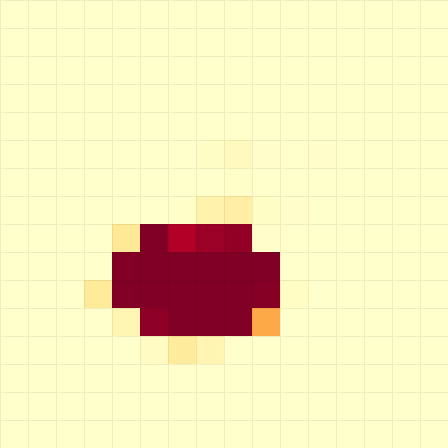
\includegraphics[width=0.78cm]{img/ev_grid.png}};
\draw[flow] (evh.east) -- (map.west);
\node[anchor=north, lbl, inner sep=1.5pt] at (map.south) {map $\hat m$\\[-1pt]\shp{16×16}};
\node[thumb] (fp) at (7.8,0.45) {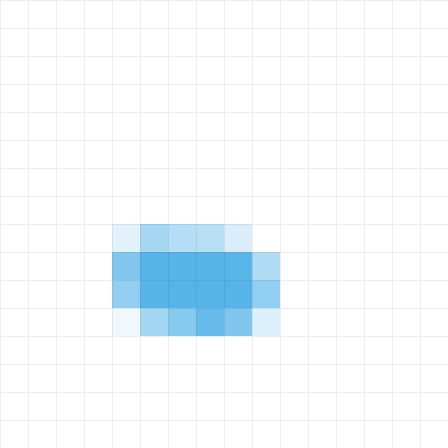
\includegraphics[width=0.78cm]{img/footprint16.png}};
\node[anchor=north, lbl, inner sep=1.5pt] at (fp.south) {footprint $M$\\[-1pt]\textcolor{muted}{target, exact}};
\draw[<->, draw=ink, line width=0.5pt] (map.east) -- node[above, font=\tinyf, text=muted, inner sep=1.2pt]{BCE} node[below, font=\tinyf, text=muted, inner sep=1.2pt]{+ Dice} (fp.west);
\end{tikzpicture}
\end{document}
